\documentclass{scioly-exam-template-araneesh}

\newcommand{\printdoctype}{Images}
\contourlength{0.15em}
\setlength{\fboxsep}{0pt}

\begin{document}
\begin{center}

% == Images Content ==
% `x' and `y' args in square brackets define the coordinate plane (i.e. 1in units relative to top left corner)
% `labelnode` args are 1. label rightward offset 2. label downward offset 3. text to display as label
\vspace*{8em}
\begin{tikzpicture}[x=1in,y=-1in]
    \imagenode{
\includegraphics[width=3in,height=3in,keepaspectratio]{images/Image1example.png}};
    \labelnode{0.3}{0.3}{1};
\end{tikzpicture}
\hspace{0.5in}
\begin{tikzpicture}[x=1in,y=-1in]
    \imagenode{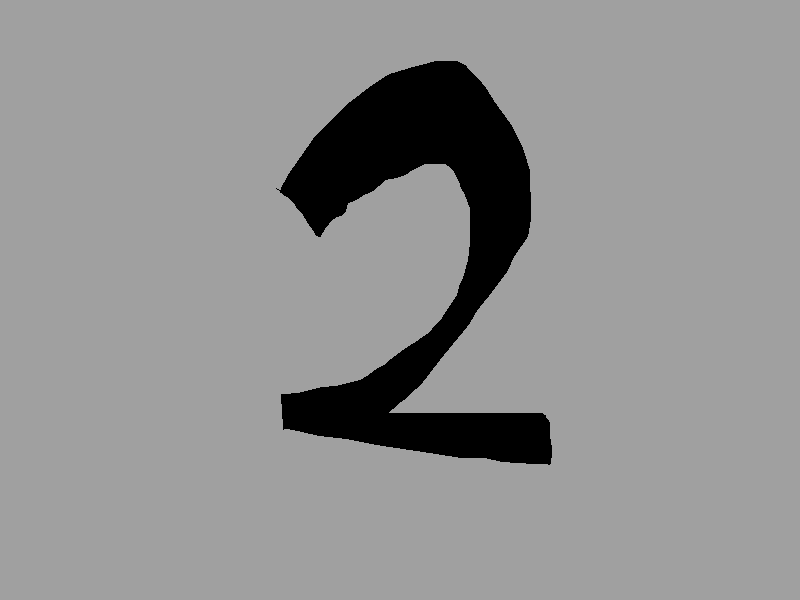
\includegraphics[width=3in,height=3in,keepaspectratio]{images/Image2example.png}};
    \labelnode{0.3}{0.3}{2};
\end{tikzpicture}
\\\vspace{0.5in}
\begin{tikzpicture}[x=1in,y=-1in]
    \imagenode{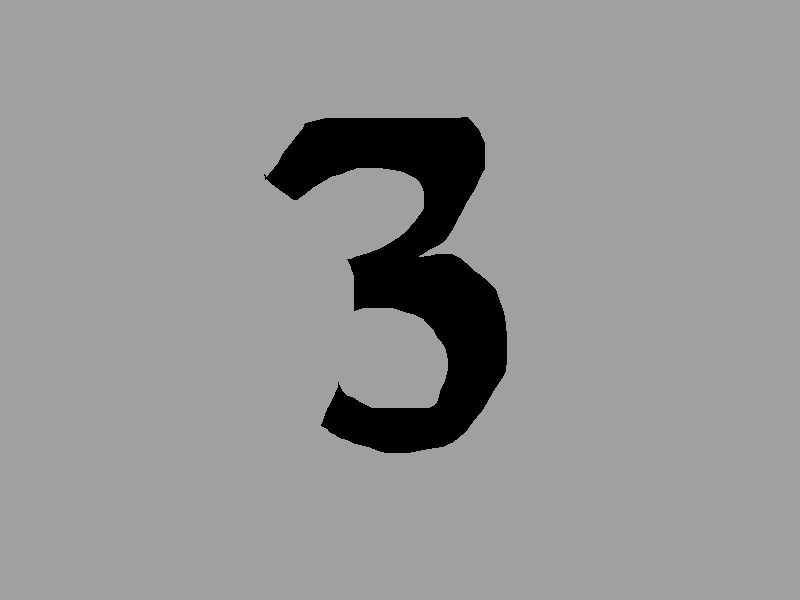
\includegraphics[width=7in,height=4in,keepaspectratio]{images/Image3example.png}};
    \labelnode{0.3}{0.3}{3};
\end{tikzpicture}
%\vfill\null
%\pagebreak

% == Closer == 
\vfill\null

\end{center}
\end{document}
